\newpage
\section{Serie numeriche}
Sia $\{a_n\}$ una successione $S\to \mathbb{R}$ una successione $S\to \mathbb{R}$. Vogliamo definire $\sum\limits_{n\in S}a_n$, la somma di tutti i termini della successione.
\begin{example}
Dato $a_n = \frac{1}{2^n}$, con $S= \{n \geq 1\}$. Voglio definire $a_1 + a_2 + a_3 + ... + a_n$.\\
Questo sarà uguale a $\frac{1}{2} + \frac{1}{4} + \frac{1}{8} + \frac{1}{16} + ... + \frac{1}{2^n}$.
\end{example}
\begin{wrapfigure}[4]{r}{6cm}
    \vspace{-25pt}
    \centering
    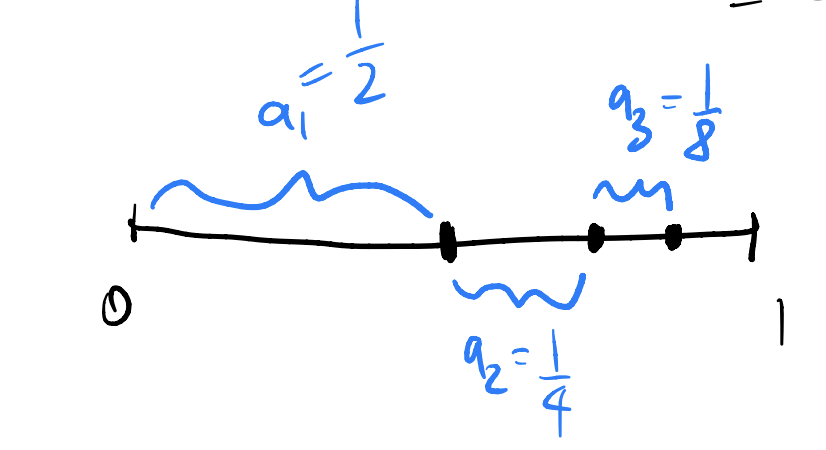
\includegraphics[width=4.7cm]{images/serie-numeriche.png}
\end{wrapfigure}
 Notiamo che aggiungendo termini sembra che la somma si avvicini sempre di pi a 1. In effetti si ha che $\frac{1}{2} + \frac{1}{4} + \frac{1}{8} + \frac{1}{16} + ... + \frac{1}{2^n} = 1 - \frac{1}{2^n}$.\\
Prendendo il limite per $n\to +\infty$ sembra ragionevole che $\frac{1}{2} + \frac{1}{4} + \frac{1}{8} + \frac{1}{16} + ... + \frac{1}{2^n} = 1$.\\

\begin{definition}
Dato $\{a_n\}: \mathbb{N} \to \mathbb{R}$, definiamo $s_n = \sum^n_{j=0}a_j = a_0 + a_i + ... + a_n$ (somma parziale n-esima), se $\{s_n\}_{n\in \mathbb{N}}$ è una nuova successione. Definiamo $\sum_{n}a_n$ (questa è la serie associata alla successione $\{a_n\}$) come $s = \lim\limits_{n\to +\infty}s_n$, se questo esiste. 
\begin{itemize}
    \item Se il limite non esiste, si dice che la serie è indeterminata.
    \item Altrimenti, se $s \in \mathbb{R}$, si dice che la serie è convergente.
    \item Mentre se $s = +\infty$ si dice che la serie diverge positivamente.
    \item Mentre se $s = -\infty$ si dice che la serie diverge negativamente.
\end{itemize}
\end{definition}

\begin{example}
Vediamo alcuni esempi di serie.
\begin{itemize}
    \item $a_n = 0 \: \forall \: n \in \mathbb{N}$, $s_n = a_0 + a_1 + ... + a_n = 0 + ... + 0 = 0$ e $s = \lim\limits_{\to +\infty}s_n = \lim\limits_{n\to +\infty}0 = 0$
    \item $a_n = 1 \: \forall \: n \in \mathbb{N}$, $s_n = a_0 + a_1 + ... + a_n = 1 + ... + 1 = n+1$ e $ s = \lim\limits_{\to +\infty}s_n = \lim\limits_{n\to +\infty}(n+1) = +\infty$.
    \item $a_n = n$, $s_n = 0 + 1 + 2 + ... + n = \frac{n(n+1)}{2}$ e quindi $\sum\limits_{n\in \mathbb{N}}a_n = \lim\limits_{n\to +\infty}s_n = \lim\limits_{n\to + \infty}\frac{n^2 + n}{2} = +\infty$.
\end{itemize}
\end{example}

\subsection{Serie geometrica}
Prendiamo un $\alpha \in \mathbb{R}$, $a_n = \alpha^n$ (l'esempio di sopra è $\alpha = \frac{1}{2}$). Proviamo ora a calcolare $\sum\limits_{n\in \mathbb{N}}a_n = \sum\limits_{n\in \mathbb{N}}\alpha^n$.\\\\
Per farlo dobbiamo calcolare le serie parziali $s_n = \sum\limits_{j=0}^n a_j = 1 + \alpha + \alpha^2 + ... + \alpha^n = \frac{\alpha^{n+1} - 1}{\alpha -1}$. Questa può essere dimostrata per induzione oppure usando la seguente uguaglianza: $x^{n+1} - y^{n+1} = (x - y)(x^n + x^{n-1}y + x^{n-1}y^2 + ... + xy^{n-1} + y^n)$.\\
Facciamo $\lim\limits_{n\to +\infty}s_n = \lim\limits_{n\to +\infty}\frac{a^{n+1}-1}{\alpha - 1}$ e questo può fare:
\begin{itemize}
    \item Se $|\alpha| < 1$, abbiamo $\alpha^{n+1}\to 0$, quindi $\sum_{n\in \mathbb{N}}\alpha^n = \lim\limits_{n\to +\infty}s_n = \lim\limits_{n\to +\infty}\frac{a^{n+1}-1}{\alpha - 1} = \frac{-1}{\alpha - 1} = \frac{1}{1 - \alpha}$. Quindi converge.
    \item Se $|\alpha| > 1$, allora $\alpha^{n+1}\to +\infty$, quindi $\sum_{n\in \mathbb{N}}\alpha^n = \lim\limits_{n\to +\infty}s_n = \lim\limits_{n\to +\infty}\frac{a^{n+1}-1}{\alpha - 1} = +\infty$, quindi diverge positivamente.
    \item Se $\alpha = 1$ allora $a_n = \alpha^n = 1^n = 1 \forall \: n \in \mathbb{N}$, quindi $\sum_{n\in \mathbb{N}}\alpha^n = \sum_{n\in \mathbb{N}}1 = +\infty$.
    \item Se $\alpha = 0$, $a_n = \alpha^n = 0 \: \forall \: n \geq 1$, quindi $\sum_{n\in \mathbb{N}}\alpha^n = \sum_{n\in \mathbb{N}}0 = 0$ quindi converge.
    \item Se $\alpha < -1$, $\alpha^{n+1}$ non ha limite e questo perché se n è pari (quindi n+1 è dispari) $\alpha^{n+1} < 0$ tende a $-\infty$ (perché $|\alpha| >1$).\\
    Se n è dispari (quindi n+1 è pari) abbiamo che $\alpha^{n+1} > 0$ e tende a $+\infty$. Abbiamo quindi due sottosuccessioni $d_{2n} \to -\infty$ e $d_{2n+1}\to -\infty$ e segue per i teoremi precedentemente visti che $b_n = \alpha^{n+1}$ non ha limite. Quindi anche $s_n = \frac{a^{n+1}-1}{\alpha - 1}$ non ha limite. \\
    $s_{2n} = \frac{b_{2n} - 1}{\alpha - 1} \to \frac{-\infty}{\alpha - 1} = +\infty$, $s_{2n+1} = \frac{b_{2n+1} - 1}{\alpha - 1} \to \frac{+\infty}{\alpha - 1} = -\infty$. Dunque $s_n$ non ha limite e $\sum_{n\in \mathbb{N}}\alpha^n$ è indeterminata se $\alpha < -1$.
    \item $\alpha = -1$, $\alpha^n = (-1)^n = \begin{cases}1 & \text{ n pari}\\ -1 & \text{ n dispari}\end{cases}$\\
    $s_0 = a_0 = (-1)^0 = 1$, $s_1 = a_0 + a_1 = 1 + (-1)^1 = 0$, $s_2 = a_0 + a_1 + a_2 = 1 + (-1)^1 + 1 = 1$, $s_3 = a_0 + a_1 + a_2 + a_3 = 1 + (-1) + 1 + (-1) = 0$ ...\\\\
    $s_n = \begin{cases}1 & \text{ n pari}\\ 0 & \text{ n dispari}\end{cases}$ non ha limite, anche in questo caso $\sum_{n\in \mathbb{N}}(-1)^n$ è indeterminata.
\end{itemize}
Riassumendo questi esempio possiamo dire che $\sum\limits_{n=0}^{+\infty}\alpha^n$:
\vspace{-15pt}
\begin{itemize}
    \item Se $|\alpha| < 1$ allora fa $\frac{1}{1 - \alpha}$.
    \item Se $\alpha \geq 1$ allora fa $+\infty$.
    \item Se $\alpha \leq 1$ allora è indeterminata.
\end{itemize}
Ora chiediamoci cosa fa $\sum_{n=k}^{+\infty}\alpha^n = \alpha^k + \alpha^{k+1} + \alpha^{k+2} + ...$ (per $|\alpha| < 1$ con $\alpha \neq 0$) \\$= \alpha^k (1 + \alpha + \alpha^2 + ...) = \frac{\alpha^k}{1 - \alpha}$. Ad esempio se $\alpha = \frac{1}{2}$ e $k=1$, quindi guardo $\frac{1}{2} + \frac{1}{4} + \frac{1}{8} + ... = \frac{\alpha^k}{1 - \alpha} = \frac{(\frac{1}{2})^1}{1 -\frac{1}{2}} = \frac{\frac{1}{2}}{\frac{1}{2}} = 1$ (come ci asoettavamo).\\\\
Invece $\sum_{n=0}^{+\infty}(\frac{1}{2})^4 = 1 + \frac{1}{2} + \frac{1}{4} + ... = 1 + 1 = 2$ ($= \frac{1}{1 - \alpha}$ in questo caso $\alpha = \frac{1}{2}$ quindi $= \frac{1}{1 - \frac{1}{2}} = \frac{1}{\frac{1}{2}} = 2$).

\begin{example}
Prendiamo $\alpha = -\frac{1}{3}$, e con $k = 0$, quindi ho $\sum_{n=0}^{+\infty}(-\frac{1}{3})^n = \frac{1}{1 + \frac{1}{3}} = \frac{3}{4}$.
\end{example}

\begin{observation}
Se $-1 < \alpha < 0$, la somma $\sum_{n=0}^{+\infty}\alpha^n = \frac{1}{1 - \alpha}$. Vediamo che $0 < -\alpha < 1 \Longrightarrow 1 < 1 - \alpha < 2$ quindi la somma è compresa tra $\frac{1}{2}$ e 1. \\
Quindi $\sum_{n=0}^{+\infty} \alpha^n = 1 + \alpha + \alpha^2 + \alpha^3 + \alpha^4 + ...$, i vari elementi sono tutti $\alpha > 0, \alpha^2 > 0, \alpha^3 > 0 \alpha^4 > 0$.
\end{observation}

\begin{example}
Un caso per calcolare il valore preciso di una serie è quando si può usare gli sviluppi di taylor. Vediamo per esempio $\sum_{n}\frac{1}{n!}$ che converge ed è uguale a $e$.\\
Partiamo da $e^x = \sum_{j=0}^n \frac{x^j}{j!} + R_n(x)$ sviluppo di taylor di $e^x$ con io resto di lagrange che in generale è $R_n = \frac{f^{n+1}(z)}{(n+1)!}(x - x_0)^{n+1}$ con z compresa tra $x$ e $x_0$.\\
Nel nostro caso $R_n(x) = \frac{e^z}{(n+1)!}(x-0) = \frac{e^z}{(n+1)!}\cdot x^n$ con z compreso tra 0 e x. Ora specifichiamo $x=1$, troviamo $e^1 = \sum_{j^0}^n \frac{1}{j!} + R_n(1) = \frac{e^z}{(n+1)}\cdot 1$. (Ricordiamo che $\sum_{j^0}^n = s_n$ per $\sum_n \frac{1}{n!}$).\\
Quindi ricavo che $|e - s_n| = \frac{e^z}{(n+1)!}$ (la z dipende da $n!$ ma è sempre $0 < z < 1$) quindi posso dire che $\frac{e^z}{(n+1)!} < \frac{e}{(n+1)!}$ Prendo il limite per $n\to +\infty$, visto che $\frac{e}{(n+1)!} \to 0$ e quindi concludo che $s_n \to e$. Quindi concludo che $\sum_{n=0}^{+\infty} \frac{1}{n!} = e$.
\end{example}

\subsection{Condizione necessaria per l'esistenza di una serie}
\begin{theorem}[Condizione necessaria di una serie]
Se $a_n$ è una successione qualsiasi, e $\sum_n a_n$ converge, allora concludo che $\lim\limits_{n\to +\infty}a_n = 0$.
\end{theorem}

\begin{demostration}
$s_{n+1} = a_0 + a_1 + a_2 + ... + a_n + a_{n+1} = s_n + a_{n+1}$. Quindi se $s_{n+1} - s_n = a_{n+1}$. Se suppongo che $\sum_n a_n = l \in \mathbb{R}$ allora $s_{n+1} - s_n \to (l - l) = 0$, ma differenza $s_{n+1} - s_n = a_n$ quindi segue che $a_n \to 0$. $\blacksquare$
\end{demostration}

\hspace{-15pt}La conseguenza pratica di questo teorema è che se ho una successione $\{a_n\}$ e controllo che $\lim\limits_{n\to +\infty}a_n$ non è 0 (quindi può non esistere oppure essere $\pm \infty$ o essere un numero $\neq 0$) allora sicuramente $\sum_n a_n$ non converge.

\begin{example}
Alcuni esempio in cui è utile usare questo teorema.
\begin{itemize}
    \item $a_n = 1 \: \forall \: n \in \mathbb{N}$. $\lim\limits_{n \in \mathbb{N}}a_n = \lim\limits_{n\to +\infty} 1 = 1$, quindi $\sum_{n\in \mathbb{N}}$ non converge.
    \item $a_n = n$, $\lim\limits_{n\to +\infty} a_n = +\infty \Longrightarrow \sum_{n\in \mathbb{N}}n$ non converge.
\end{itemize}
\end{example}

\hspace{-15pt}Attenzione che se $\lim\limits_{n\to +\infty}a_n = 0$, non è detto che $\sum_n a_n$ converga.

\subsection{Valore della somma di sue serie}
\begin{theorem}
se $a_n$ e $b_n$ sono due successioni e $\sum_{n}a_n$ e $\sum_n b_n$ hanno senso (cioè non sono indeterminate) allora anche $\sum_n (a_n + b_n)$ ha senso e vale $\sum_n (a_n + b_n) = \sum_n a_n + \sum_n b_n$ questo supponendo che la somma non sia una forma indeterminata.\footnote{Le forme indeterminate possibili sono $+\infty - \infty$ o $-\infty + \infty$}
\end{theorem}

\begin{example}
Alcuni esempi di utilizzo di questo teorema.
\begin{itemize}
    \item $a_n = (\frac{1}{2})^n$, $b_n = (\frac{1}{3})^n$. Abbiamo $\sum^{+\infty}_{n=0}a_n = \frac{1}{1 - \frac{1}{2}} = 2$, $\sum^{+\infty}_{n=0}b_n = \frac{1}{1 - \frac{1}{3}} = \frac{3}{2}$. \\
    Quindi $\sum_{n=0}^{+\infty}(a_n + b_n) = \sum_{n=0}^{+\infty}((\frac{1}{2})^n + (\frac{1}{3})^n) = 2 + \frac{3}{2} = \frac{7}{2}$.
    \item $a_n = 1$, $b_n = -1$, ho $\sum_n a_n = +\infty$, $\sum_n b_n = -\infty$ quindi $\sum_n (a_n + b_n)$ non si può sapere tramite il teorema perché non si applica. Però $a_n + b_n = 1 - 1 = 0$, quindi $\sum_n (a_n + b_n) = 0$.
    \item $a_n = n^2$, $b_n = -n$, ho quindi $\sum_n a_n = +\infty$, $\sum_n b_n = -\infty$. Questa volta $a_n + b_n = n^2 - n \to +\infty$ (perché $n^2 - n = n(n-1)$) e segue dalla condizione necessaria che $\sum_n (a_n + b_n)$ non converge (ma diverge positivamente, visto che $a_n + b_n \to +\infty$).
\end{itemize}
\end{example}

\begin{observation}
Non c'è un teorema analogo riguardo a $\sum_n (a_n \cdot b_n)$. In particolare non è vero che $\sum_n(a_n \cdot b_n) = (\sum_n a_n) \cdot (\sum_n b_n)$.
\end{observation}

\begin{example}
Possiamo vedere del perché di questa osservazione prendendo $a_n = (\frac{1}{2})^n$, $b_n = (\frac{1}{3})^n$. $\sum_n a_n = 2$, $\sum_n b_n = \frac{3}{2}$. $a_n \cdot b_n = (\frac{1}{6})^2$ e $\sum_n a_n \cdot b_n = \sum_n (\frac{1}{6})^n = \frac{1}{1 - \frac{1}{6}} = \frac{6}{5}$ e $\frac{6}{5} \neq 2 \cdot \frac{3}{2}$.
\end{example}

\hspace{-15pt}Può anche succedere che $\sum_n a_n$ e $\sum_n b_n$ convergano ma $\sum_n a_n \cdot b_n$ non converge.

\subsection{Serie definitivamente a termini positivi}
\begin{theorem}
Se ho $a_n \geq 0$ definitivamente \footnote{Questo vuol dire che da un certo punto in poi è sempre positiva} allora $\sum_n a_n$ converge oppure diverge positivamente (non pu essere indeterminata o andare a $-\infty$).
\end{theorem}

\begin{demostration}
Come prima abbiamo visto che $s_{n+1} = s_n + a_{n+1}$. Se $a_n \geq 0$ definitivamente, ho che $s_{n+1} \geq s_n$ definitivamente. Quindi $\{s_n\}$ è definitivamente (debolmente) crescente, quindi ammette limite, che può essere un numero reale, oppure $+\infty$ (non $-\infty$ perchè ho una successione che sta crescendo). $\blacksquare$
\end{demostration}

\begin{observation}
Se $a_n \leq 0$ definitivamente, analogamente si può dire che $\sum_n a_n$ converge oppure diverge negativamente.
\end{observation}

\subsection{Criterio del confronto}
\begin{theorem}[Criterio del confronto]
Se $o \leq a_n \leq b_n$ definitivamente. Allora:
\begin{enumerate}
    \item Se $\sum_n b_n$ converge $\Longrightarrow \sum_n a_n$ converge.
    \item Se $\sum_n a_n$ diverge $\Longrightarrow \sum_n b_n$ diverge. 
\end{enumerate}
\end{theorem}

L'idea è che se $0 \leq a_n \leq b_n \: \forall \: \in \mathbb{N}$, allora $0 \leq \sum_n a_n \leq \sum_n b_n$

\begin{example}
Alcuni esempi su questo teorema.
\begin{itemize}
    \item Sapendo che $\sum_n 1 = +\infty$, posso concludere che $\sum_{n=0}^{+\infty}n = +\infty$ (perché $0 \leq 1 \leq n \forall \: n \geq 1$) e anche $\sum_{n=0}^{+\infty}n^2 = +\infty$ (perché $0 \leq 1 \leq n^2 \: \forall \:n \geq 1$)
    \item Voglio sapere cosa fa $\sum_n \frac{\sin{n}^2}{2^2}$. $a_n = \frac{\sin{n}^2}{2^n} \leq \frac{1}{2^n} = b_n$. So che $\sum_n b_n$ converge e sappiamo calcolare la somma, dunque per il teorema anche questa $\sum_n a_n$ converge.
    \item Cosa fa $\sum_n n!$. Abbiamo $n! \geq n \: \forall \:n \geq 1$, e sappiamo che $\sum_n n = +\infty$, quindi concludiamo che $\sum_n n! = +\infty$
\end{itemize}
\end{example}

\subsection{Criterio del confronto asintotico}
\begin{theorem}[Criterio del confronto asintotico]
Prendiamo $\{a_n\}, \{b_n\}$ successioni, tale che $a_n > 0$ e $b_n > 0$ definitivamente, e supponiamo che $\lim\limits_{n\to +\infty}\frac{a_n}{b_n}= l \in \overline{\mathbb{R}}$. Allora si può dire che:
\begin{enumerate}
    \item Se $l \in (0, +\infty)$, allora $\sum_n a_n$ e $\sum_n b_n$ hanno lo stesso comportamento (cioè entrambe convergono o entrambe divergono a $+\infty$).
    \item Se $l = 0$ e $\sum_n b_n$ converge allora $\sum_n a_n$ converge. ("infatti" $\frac{a_n}{b_n}\to 0 \Longrightarrow \frac{a_n}{b_n} <1$ definitivamente $\Longrightarrow a_n < b_n$ definitivamente e da qui è chiaro che $se \sum_n b_n$ converge allora anche $\sum_n a_n$)
    \item Se $l = +\infty$ e $\sum_n b_n$ diverge, allora $\sum_n a_n$ diverge. ($\frac{a_n}{b_n}\to +\infty \Longrightarrow \frac{a_n}{b_n} > 1$ definitivamente $\Longrightarrow a_n > b_n$ definitivamente)
\end{enumerate}
\end{theorem}

\begin{observation}
Ad esempio nel punto (2), se $\sum_n b_n = +\infty$, non posso concludere niente riguardo a $\sum_a a_n$.
\end{observation}

\begin{example}
$\sum_n \frac{1}{2^n - \log(n)}$. $a_n = \frac{1}{2^n - \log(n)}$, definitivamente $> 0$ perché $2^n > \log(n)$ definitivamente. L'idea qui è che per n grande, $\log(n)$ "conta molto meno di $2^n$" quindi faccio confronto asintotico con $b_n = \frac{1}{2^n}$.\\
Abbiamo $\lim\limits_{n\to +\infty}\frac{a_n}{b_n} = \lim\limits_{n\to +\infty} \frac{\frac{1}{2^n - \log(n)}}{\frac{1}{2^n}} = \lim\limits_{n\to +\infty}\frac{2^n}{2^n - \log(n)} = \lim\limits_{n\to +\infty} \frac{1}{1 - \frac{\log(n)}{2^n}} = 1$ questo è l. Quindi in questo caso $l \in (0, +\infty)$, quindi $\sum_n a_n$ ha lo stesso comportamento di $\sum_n b_n = \sum_n (\frac{1}{2})^n$ che converge. Quindi $\sum_n a_n$ converge.
\end{example}

\subsection{Criterio della radice}
\begin{theorem}[Criterio della radice]
Prendo una $\{a_n\}$ una successione tale che $a_n > 0$ definitivamente. Se $\exists \: \lim\limits_{n \to +\infty}\sqrt[n]{a_n} = l \in \overline{\mathbb{R}}$.
\begin{enumerate}
    \item Se $0 \leq l \leq 1$, allora $\sum_n a_n$ converge. ($\Longrightarrow$ per la condizione necessaria $\lim\limits_{n\to +\infty}a_n = 0$).
    \item Se $l > 1$, allora $\sum_n a_n$ diverge.
\end{enumerate}
\end{theorem}

\begin{demostration}
Dimostriamo i due casi del teorema.
\begin{enumerate}
    \item Se $l < 1$, scelgo $\alpha \in \mathbb{R}$ tale che $l < \alpha < 1$, e visto che $\sqrt[n]{a_n}\to l$, definitivamente avrò $\sqrt[n]{a_n} < \alpha$ quindi $a_n < \alpha^n$ definitivamente. Per confronto, visto che $\sum_n \alpha^n$ converge, concludo che anche $\sum_n a_n$ converge.
    \item Discorso simile anche per questo punto, quindi prendo $< \alpha < l$, e poi definitivamente $\alpha < \sqrt[n]{a_n}$ quindi $\alpha^n < a_n$ definitivamente, e ora però $\sum_n \alpha^n = +\infty$ perché $\alpha > 1$, quindi anche $\sum_n a_n$ diverge. $\blacksquare$
\end{enumerate}
\end{demostration}

\begin{observation}
Come per le successioni quando $l=1$ no si può concludere niente.
\end{observation}

\begin{example}
$\sum_n \frac{n}{3^n}$, $a_n = \frac{n}{3^n}$, e $\sqrt[n]{a_n} = \frac{\sqrt[n]{n}}{3} \to \frac{1}{3} = l$ quindi $l < 1$, e quindi la serie converge.
\end{example}

\newpage
\subsection{Criterio del rapporto}
\begin{theorem}[Criterio del rapporto]
Prendo $\{a_n\}$ successione, $a_n > 0$ definitivamente. Se $\exists \lim\limits_{n \to +\infty}\frac{a_{n+1}}{a_n} = l \in \overline{\mathbb{R}}$.
\begin{enumerate}
    \item Se $0 \leq l < 1$, allora $\sum_n a_n$ converge.
    \item Se $l > 0$, allora $\sum_n a_n$ diverge.
\end{enumerate}
\end{theorem}

\begin{demostration}
Sappiamo che se $\exists \: \lim\limits_{n\to +\infty}\frac{a_{n+1}}{a_n} = l$, allora esiste anche $\lim\limits_{n\to +\infty}\sqrt[n]{a_n}$, ed è uguale a l. Quindi la conclusione segue dal criterio della radice (appena visto).
\end{demostration}

\begin{example}
$\sum_n \frac{n^2}{n!}$, $a_n = \frac{n^2}{n!}$. Usiamo il criterio del rapporto.\\
$\frac{a_{n+1}}{a_n} = \frac{(n+1)^2}{(n+1)!} \cdot \frac{n!}{n^2} = \frac{(n+1)^2}{(n+1)n!}\cdot \frac{n!}{n^2} = \frac{n+1}{n^2} \to 0 = l$. Quindi visto che $l = 0$, concludo che la serie converge.
\end{example}

\begin{observation}
Questi criteri per successioni definitivamente positive si applicano anche a successioni \textbf{definitivamente negative}. Infatti se $a_n < 0$ definitivamente allora $-a_n > 0$ definitivamente, quindi applico i criteri visti alla successioni $\{-a_n\}$ e poi $\sum_{j=0}^n a_j = -\sum_{j=0}^n(-a_j)$ dunque $\sum_{n=0}^{+\infty}a_n = -\sum_{n=0}^{+\infty}(-a_n)$ (se i limiti esistono).
\end{observation}

\subsection{Legami con gli integrali impropri}
Una serie $\sum_n a_n$ si può scrivere come integrale improprio. Considero una $f: [0,+\infty) \to \mathbb{R}$ data da $f(x)=a_{[x]}$ ($[x]$ parte intera di un x).\\
\begin{wrapfigure}[4]{r}{6cm}
    \vspace{-33pt}
    \centering
    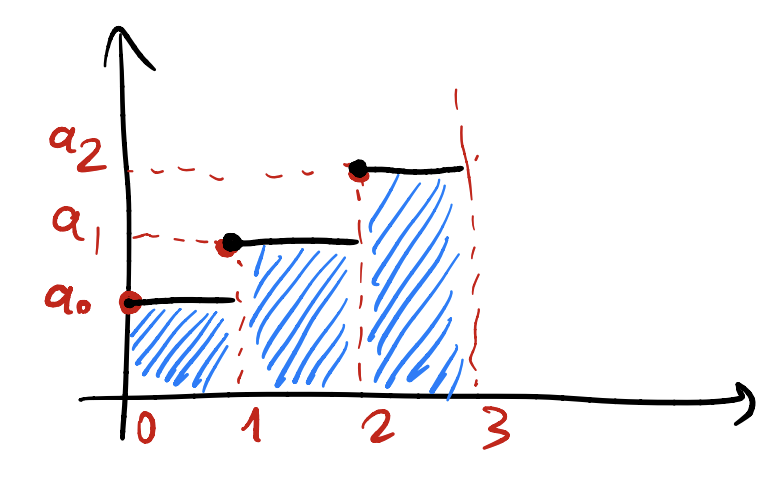
\includegraphics[width=5cm]{images/legame-serie-integrali-impropri.png}
\end{wrapfigure}
Si crea dunque una funzione a gradini. Si ha $\sum_{j=0}^n a_j = \int_0^{n+1}f(x)\:dx$. Quindi prendendo il limite per $n\to +\infty$, trovo $\sum_n a_n = \int_0^{+\infty}f(x)\:dx$ (se i limiti hanno senso).\\\\
\begin{wrapfigure}[5]{l}{6cm}
    \vspace{-30pt}
    \centering
    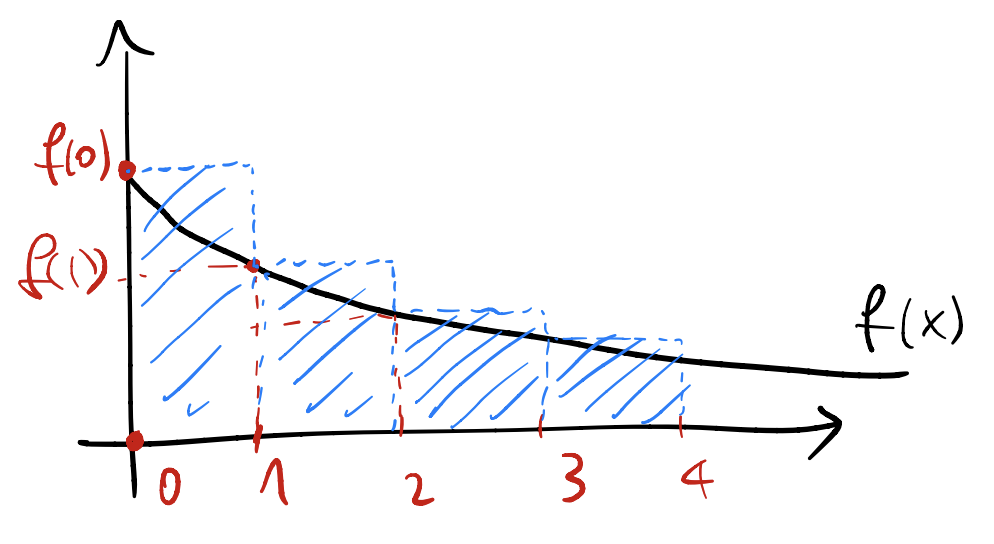
\includegraphics[width=5.5cm]{images/legame-serie-integrali-impropri-2.png}
\end{wrapfigure}

Viceversa, partendo da  $f: [0,+\infty)\to \mathbb{R}$, posso considerare la successione $a_n = f(n)$ e la serie $\sum_n a_n = \sum_n f(n)$ (in questo caso la serie $\sum_n a_n$ è la somma delle aree dei rettangoli blu). Questa volta $\sum_n a_n$ e $\int_0^{+\infty}f(x) \:dx$ non saranno proprio uguali.\\
\begin{theorem}[Criterio dell'integrale]
Fissiamo $\overline{n} \in \mathbb{N}$, e $f: [\overline{n}, +\infty) \to \mathbb{R}$ che sia debolmente crescente, continua, con $f(x) \geq 0 \: \forall x \in [\overline{n}, +\infty)$, e poniamo $a_n = f(n)$. Allora $\sum_n a_n$ e $\int_{\overline{n}}^{+\infty}f(x)\:dx$ hanno lo stesso comportamento, e $\sum_{n=\overline{n}+1}^{+\infty}$.
\end{theorem}
Questo teorema può essere usato per entrambi i versi.
\begin{example}
Vediamo alcuni esempi del criterio.
\begin{itemize}
    \item $\sum_n \frac{1}{n^{\alpha}}$. Serie armonica generalizzata ($\alpha = 1 \longrightarrow \sum_n \frac{1}{n}$ serie armonica).\\
    Converge se $\alpha > 1$, e dunque se $\alpha \leq 1$. Infatti se prendo $f(x) = \frac{1}{x^{\alpha}}$ è decrescente e continua.
    Quindi abbiamo che $\int_1^{+\infty}\frac{1}{x^{\alpha}}$:
    \begin{itemize}
        \item Converge se $\alpha > 1$.
        \item Diverge a $+\infty$ se $\alpha \leq 1$
    \end{itemize}
    Quindi applicando il criterio dell'integrale si conclude quello scritto sopra.
    \begin{observation}
    Se $\alpha \leq 0$, $\sum_n\frac{1}{x^{\alpha}}$ diverge perché non è soddisfatta nemmeno la condizione necessaria.
    \end{observation}
    \item Calcoliamo $\sum_{n=2}^{+\infty}\frac{1}{n^{\alpha}(\log(n))^{\beta}}$. Usiamo il criterio dell'integrale con $f(x) = \frac{1}{x^{\alpha}(\log(x))^{\beta}}$.\\
    $\int_2^{+\infty}\frac{1}{x^{\alpha}(\log(x)^{\beta}}$ posiamo notare che:
    \begin{itemize}
        \item Converge se $\alpha > 1$, $\beta \in \mathbb{R}$.
        \item Diverge se $\alpha < 1$, $\beta \in \mathbb{R}$.
        \item Converge se $\alpha = 1$, $\beta > 1$.
        \item Diverge se $\alpha = 1$, $\beta \leq 1$.
    \end{itemize}
    (Questo come visto in precedenza). La serie si comporta allo stesso modo.
\end{itemize}
\end{example}

\begin{example}
Prendiamo $\sum_{n=1}^{+\infty}(e^{\frac{1}{n}} - 1)$. $a_n = e^{\frac{1}{n}} - 1 > 0$ (essendo maggiore di zero posso usare in seguito il confronto asintotico).\\
$\lim\limits_{n\to +\infty}a_n = \lim\limits_{n\to +\infty}(e^{\frac{1}{n}}-1) = e^0 - 1 = 1 - 1 = 0$. Quindi la condizione necessaria è soddisfatta e la serie può convergere. Possiamo usare lo sviluppo di talyor con $e^t = 1 + t + o(t)$ per $t\to 0$, quindi $e^{\frac{1}{n}} = 1 + \frac{1}{n} + \frac{1}{n}$ (t = $\frac{1}{n}$).
In termini di "importante" sarà $\frac{1}{n}$. In questi casi pongo $b_n = \frac{1}{n}$ e uso il confronto asintotico:\\
$\lim\limits_{n \to +\infty}\frac{a_n}{b_n} = \lim\limits_{n \to +\infty}\frac{e^{\frac{1}{n}}-1}{\frac{1}{n}} = \lim\limits_{n \to +\infty} \frac{\frac{1}{n} + o(\frac{1}{n})}{\frac{1}{n}} = \lim\limits_{n \to +\infty}(1 + o(1)) = 1$. \\
Per confronto asintotico, concludo che $\sum_n a_n$ ha lo stesso comportamento di $\sum_n b_n = \sum_n \frac{1}{n}$ (che è la serie armonica) che sappiamo diverge. Quindi $\sum_n a_n$ diverge a $+\infty$.
\end{example}

\subsection{Convergenza assoluta}
Prendiamo $\{a_n\}$ un successione qualsiasi (quindi non supponiamo che sia ne definitivamente positivo ne def. negativo).
\begin{definition}[Convergenza assoluta]
Diamo che $\sum_n a_n$ \textbf{converge assolutamente} se $\sum_n |a_n|$ converge.
\end{definition}

\begin{theorem}[Criterio dell'assoluta convergenza]
Se la serie $\sum_n a_n$ converge assolutamente, allora converge, e $|\sum_n a_n| \leq \sum_n |a_n|$.
\end{theorem}

\begin{demostration}
Dimostrazione che segue quella dell'analogo per gli integrali impropri. Vediamo innanzitutto che $a_n = a_n^+ - a_n^-$, mentre $|a_n| = a_n^+ + a_n^-$ e $0 \leq a_n^+ \leq |a_n|$, $0 \leq a_n^- \leq |a_n|$ e se $\sum_n |a_n|$ converge, per confronto convergono anche $\sum_n a_n^+$ e $\sum_n a_n^-$. Quindi converge anche $\sum_n a_n = \sum_n a_n^+ - \sum_n a_n^-$. Per la disuguaglianza triangolare se prendo $|\sum_{j=0}^n a_j| \leq \sum_{j=0}^n |a_j|$ e prendendo il limite per $n\to +\infty$ trovo $|\sum_n a_n| \leq \sum_n |a_n|$. $\blacksquare$
\end{demostration}

\begin{example}
Prendo $\sum_{n=1}^{+\infty}\frac{\sin{n}}{n^2}$. $a_n = \frac{\sin{n}}{n^2}$ è a segno variabile. \\
$|a_n| = |\frac{\sin{n}}{n^2}| = \frac{|\sin{n}|}{n^2} < \frac{1}{n^2}$. Visto che $\sum_n \frac{1}{n^2}$ converge (serie armonica generalizzata con $\alpha = 2 > 1$) per confronto segue che $\sum_n |\frac{\sin{n}}{n^2}|$ converge, quindi per il criterio di assoluta convergenza, concludo che anche $\sum_n \frac{\sin{n}}{n^2}$ converge (notiamo che però non sappiamo a che numero converge sappiamo solo che converge).
\end{example}

\begin{observation}
Se $\sum_n |a_n|$ diverge, non si può dire niente riguardo a $\sum_n a_n$ (cioè la $\sum a_n$ potrebbe converge o divergere).
\end{observation}

\subsection{Criterio di Leibnitz}
\begin{definition}[Serie a segno alterno]
Una serie a segno alterno è una serie della forma $\sum_n (-1)^n \cdot a_n$, dove $\{a_n\}$ è una successione a segno costante.
\end{definition}

\begin{example}
$\sum_n \frac{(-1)^n}{n^3}$ è a segno alterno. $\sum_n (-1)^n(-\frac{1}{n})$ è a segno alterno.. $\sum_n (-1)^n \sin{n}$ non è a segno alterno.
\end{example}

\begin{theorem}[Criterio di Leibnitz]
Se ho $\{a_n\}$ definitivamente $\geq 0$ e debolmente crescente e tale che $\lim\limits_{n\to +\infty}a_n = 0$, allora $\sum_n (-1)^n a_n$ converge.
E $\big|\sum_{j=0}^{+\infty}(-1)^ja_j - \sum_{j=0}^{n}(-1)^j a_j \big| \leq a_{n+1}$.
\end{theorem}

\begin{example}
Vediamo alcuni esempi di questo criterio.
\begin{itemize}
    \item $\sum_n \frac{(-1)^n}{n}$ converge, perché $a_n = \frac{1}{n}$ è $\geq 0$ e debolmente decrescente e $\lim\limits_{n\to +\infty}\frac{1}{n} = 0$.\\
    Notare che la serie dei valori assoluti è $\sum_n |\frac{(-1)^n}{n}| = \sum_n \frac{1}{n} = +\infty$. Questo è un esempio in cui $\sum_n |b_n|$ diverge ma $\sum_n b_n$ converge.
    \item $\sum_n \frac{(-1)^{n+1}}{n}$ vediamo se si può applicare Laibnitz. $b_n = \frac{(-1)^{n+1}}{n} = -\frac{(-1)^n }{n}$ converge, quindi converge anche $\sum_n \frac{(-1)^{n+1}}{n} = -\sum_n \frac{(-1)^n}{n}$.
\end{itemize}
\end{example}

\begin{example}
Vediamo alcuni esempi particolari "di avvertimento".
\begin{itemize}
    \item Può essere che $\sum_n a_n$ e $\sum_n b_n$ convergano, ma $\sum_n a_nb_n$ non converga.\\
    $a_n = \frac{(-1)^n}{n}$, $b_n = \frac{(-1)^n}{\log(n)}$. $\sum_n a_n$ converge. $\sum_n b_n = \sum_{n \geq 0} \frac{(-1)^n}{\log(n)}$ converge per Leibnitz.\\
    $a_nb_n = \frac{(-1)^n}{n} \cdot \frac{(-1)^n}{\log(n)} = (-1)^{2n}\cdot \frac{1}{n\log(n)} = \frac{1}{n\log(n)}$ e $\sum_n a_nb_n = \sum_n \frac{1}{n\log(n)}$ diverge (visto prima).
    \item Il confronto asintotico non funziona se il segno della successione non è definitivamente costante.\\
    $a_n = \frac{(-1)^n}{\sqrt{n}}$, $b_n = \frac{(-1)^n}{\sqrt{n}} + \frac{1}{n} = \frac{(-1)^n \sqrt{n} + 1}{n}$. Si ha $\lim\limits_{n\to +\infty}\frac{a_n}{b_n} = \lim\limits_{n\to +\infty}\frac{\frac{(-1)^n}{\sqrt{n}}}{\frac{(-1)^n\sqrt{n}+1}{n}} = \lim\limits_{n\to +\infty} \frac{(-1)^n \sqrt{n}}{(-1)^n \sqrt{n} + 1} = \lim\limits_{n\to +\infty}\frac{1}{1 + \frac{1}{(-1)^n \sqrt{n}}} = 1$ (perché $ \frac{1}{(-1)^n \sqrt{n}} \to 0$).\\
    Quindi il confronto asintotico (se funzionasse) mi diverge che $\sum a_n$ e $\sum b_n$ hanno lo stesso comportamento. Ma $\sum_n a_n = \sum_n \frac{(-1)^n}{\sqrt{n}}$ converge per Leibnitz e $\sum_n b_n = \sum_n b_n = \sum_n \frac{(-1)^n}{\sqrt{n}} + \sum_n \frac{1}{n}$ ($\sum_n \frac{(-1)^n}{\sqrt{n}}$ converge e $\sum_n \frac{1}{n} = +\infty$) quindi $\sum_n b_n$ diverge.
\end{itemize}
\end{example}